% **************************************************
% Document Class Definition
% **************************************************
\documentclass[%
    paper=A4,               % paper size --> A4 is default in Germany
    twoside=false,           % onesite or twoside printing
    openright,              % doublepage cleaning ends up right side
    parskip=full,           % spacing value / method for paragraphs
    chapterprefix=true,     % prefix for chapter marks
    11pt,                   % font size
    headings=normal,        % size of headings
    bibliography=totoc,     % include bib in toc
    listof=totoc,           % include listof entries in toc
    titlepage=on,           % own page for each title page
    captions=tableabove,    % display table captions above the float env
    draft=false,            % value for draft version
]{scrreprt}%


% **************************************************
% Setup YOUR thesis document in this file !
% **************************************************
% !TEX root = thesis.tex


% **************************************************
% Files' Character Encoding
% **************************************************
\PassOptionsToPackage{utf8}{inputenc}
\usepackage{inputenc}


% **************************************************
% Information and Commands for Reuse
% **************************************************
\newcommand{\thesisTitle}{Topic Model Visualization for Opinion Mining}
\newcommand{\thesisTitleGer}{Topic Model Visualisierung für Opinion Mining}
\newcommand{\thesisAuthor}{Maria Potzner}
\newcommand{\thesisType}{Bachelor's Thesis}
\newcommand{\thesisDate}{15. November 2018}

\newcommand{\thesisSupervisor}{PD Dr. Georg Groh}
\newcommand{\thesisAdviser}{PD Dr. Georg Groh}

\newcommand{\thesisUniversity}{\protect{Technical University of Munich}}
\newcommand{\thesisUniversityDepartment}{Department of Informatics}
\newcommand{\thesisUniversityFaculty}{Information Systems}

% **************************************************
% Debug LaTeX Information
% **************************************************
%\listfiles


% **************************************************
% Load and Configure Packages
% **************************************************

\PassOptionsToPackage{table}{xcolor}
\usepackage[english]{babel} % babel system, adjust the language of the content
\PassOptionsToPackage{% setup clean thesis style
    figuresep=colon,%
    sansserif=false,%
    hangfigurecaption=false,%
    hangsection=true,%
    hangsubsection=true,%
    colorize=full,%
    colortheme=bluemagenta,%
    bibsys=bibtex,%
    bibfile=library,%
    bibstyle=authoryear,%
    wrapfooter=false,%
}{cleanthesis}
\usepackage{cleanthesis}



\hypersetup{% setup the hyperref-package options
    pdftitle={\thesisTitle},    %   - title (PDF meta)
    pdfsubject={\thesisType},%   - subject (PDF meta)
    pdfauthor={\thesisAuthor},    %   - author (PDF meta)
    plainpages=false,           %   -
    colorlinks=true,           %   - colorize links?
    pdfborder={0 0 0},          %   -
    breaklinks=true,            %   - allow line break inside links
    bookmarksnumbered=true,     %
    bookmarksopen=true          %
}

\usepackage{subfig}
\usepackage{tumlogo}
\usepackage{booktabs}
\usepackage{tikz}
\usepackage{tabularx}
\usepackage{ltablex}
\usetikzlibrary{bayesnet}
\usepackage{pgfplots}
\usepackage{xcolor}
\usepackage{multirow}
\usepackage{makecell}
\usepackage{amsmath,amsfonts,amssymb,amsthm}
\usepackage{rotating}
\usepackage{lineno}
\usepackage{smartdiagram}
\usepackage[printonlyused, withpage]{acronym}
%\usepackage{subcaption}
%\captionsetup[subfigure]{list=true, font=large, labelfont=bf, 
%	labelformat=brace, position=top}
\usepackage[cache=false]{minted}




% **************************************************
% Document CONTENT
% **************************************************
\begin{document}

% --------------------------
% rename document parts
% --------------------------
%\renewcaptionname{ngerman}{\figurename}{Abb.}
%\renewcaptionname{ngerman}{\tablename}{Tab.}
\renewcaptionname{english}{\figurename}{Fig.}
\renewcaptionname{english}{\tablename}{Tab.}

% --------------------------
% Front matter
% --------------------------
\pagenumbering{roman}			% roman page numbing (invisible for empty page style)
\pagestyle{empty}				% no header or footers
% !TEX root = ../my-thesis.tex
%
% ------------------------------------  --> cover title page
\begin{titlepage}
	% Should the titlepages be centered or margins like the rest of the document
	\setlength{\evensidemargin}{22pt}
	\setlength{\oddsidemargin}{22pt}
	\pdfbookmark[0]{Cover}{Cover}
	\vspace{4cm}
	\hfill
	
	\begin{center}
		\oTUM{4cm}\\ 
		\vspace{5mm}     
		\huge DEPARTMENT OF INFORMATICS\\ 
		\vspace{0.5cm}
		\large TECHNICAL UNIVERSITY OF MUNICH\\
		\vspace{1mm}
	\end{center}
	
	\vspace{13mm}
	
	\begin{center}
		{\Large \thesisType\ in \thesisUniversityFaculty}
		\vspace{20mm}
		
		\begin{spacing}{1.5}
			{\huge\bfseries \thesisTitle}\\%[3ex]
		\end{spacing}
		
		\vspace{15mm}
		{\LARGE \thesisAuthor}
		
		\vspace{20mm}
		
		\begin{figure}[h!]
			\centering
			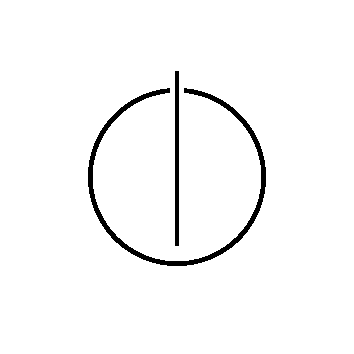
\includegraphics[width=0.3\linewidth]{gfx/infologo_BW.png}
		\end{figure}
	\end{center}
	
\end{titlepage}


% ------------------------------------  --> main title page
\begin{titlepage}
	\setlength{\evensidemargin}{22pt}
	\setlength{\oddsidemargin}{22pt}
	\pdfbookmark[0]{Titlepage}{Titlepage}
	\vspace{4cm}
	\hfill
	\begin{center}
		\oTUM{4cm}
		
		\vspace{5mm}     
		\huge DEPARTMENT OF INFORMATICS\\ 
		\vspace{0.5cm}
		\large TECHNICAL UNIVERSITY OF MUNICH\\
	\end{center}
	
	\vspace{5mm}
	
	\begin{center}
		{\Large \thesisType\ in \thesisUniversityFaculty}
		\vspace{8mm}
		
		\begin{spacing}{1.3}
			{\LARGE \thesisTitle}\\
			\vspace{8mm}
			
			{\LARGE \thesisTitleGer}\\
			\vspace{20mm}
		\end{spacing}
		
		\begin{tabular}{ll}
			\Large Author:     & \Large \thesisAuthor     \\[2mm]
			\Large Supervisor: & \Large \thesisSupervisor \\[2mm]				
			\Large Advisor:	   & \Large \thesisAdviser    \\[2mm]
			\Large Submission date:       & \Large \thesisDate
		\end{tabular}
		
		\vspace{20mm}
		
		\begin{figure}[hb!]
			\centering
			
\includegraphics[width=0.2\linewidth]{gfx/infologo.jpg}
		\end{figure}
		
	\end{center}

\end{titlepage}


% ------------------------------------  --> lower title back for single page layout
%\hfill
%\vfill
%{
%	\small
%	\textbf{\thesisName} \\
%	\textit{\thesisTitle} \\
%	\thesisSubject, \thesisDate \\
%	Reviewers: \thesisFirstReviewer\ and \thesisSecondReviewer \\
%	Supervisors: \thesisFirstSupervisor\ and \thesisSecondSupervisor \\[1.5em]
%	\textbf{\thesisUniversity} \\
%	\textit{\thesisUniversityGroup} \\
%	\thesisUniversityInstitute \\
%	\thesisUniversityDepartment \\
%	\thesisUniversityStreetAddress \\
%	\thesisUniversityPostalCode\ and \thesisUniversityCity
%}

\cleardoublepage
% !TEX root = ../my-thesis.tex
%
%************************************************
% Declaration
%************************************************
\pdfbookmark[0]{Declaration}{Declaration}
\thispagestyle{empty}

\vspace*{0.8\textheight}
\noindent
I confirm that this bachelor's thesis is my own work and I have documented all sources and material used.

\vspace{15mm}
\noindent
Munich, \thesisDate \hspace{\stretch{1}} \thesisAuthor
\newpage


%*****************************************
%*****************************************

\cleardoublepage

\pagestyle{plain}				% display just page numbers
% !TEX root = ../my-thesis.tex
%
\pdfbookmark[0]{Abstract}{Abstract}
\chapter*{Abstract}
\label{sec:abstract}
\vspace*{-10mm}

blablablub

\vspace*{20mm}

{\usekomafont{chapter} Zusammenfassung}\label{sec:abstract-diff} \\

blablablub
		% INCLUDE: the abstracts (english and german)
\cleardoublepage
%
% !TEX root = ../my-thesis.tex
%
\chapter*{Acknowledgement}
\label{sec:acknowledgement}
\vspace*{-10mm}

As this thesis borders between computer science and qualitative research on consumer behaviour I would like PD Dr. Georg Groh of the Research Group for Social Computing for his input during the project and Hannah Danner from the Chair of Marketing and Consumer behavior. Without their collaboration this project and thesis would not be possible. 

Special thanks got to my supervisor Dietrich Trautmann for his support and good ideas during the project and for the continuous reviews and feedback while I wrote this thesis. 

Furthermore, I would like to thank the other team members of the SocialROM project Adnan Akhundov, Ahmed Ayad, Tim Berger, Rajat Jain, Tim Berger, Vishesh Mathur and Adrian Philipp for often tedious but every-time fruitful discussions every week.

While writing this thesis the English Writing Center of the TUM was contacted several times. I especially like to thank the fellows Rose Jacobs,  Sean Rohringer, Hasan Ashraf, and Keefe Huang for reviewing my thesis.

I would like to use this opportunity to thank my parents Irina and Alexander as well as my brother Julian for their continued support during the first part of my studies. Further, I would like to thank Maria Potzner for her support while working on this project and for proof-reading this thesis. 

%jan hauffa, gerry hagerer, team members % INCLUDE: acknowledgement
\cleardoublepage
%
\setcounter{tocdepth}{2}		% define depth of toc
\tableofcontents				% display table of contents
\cleardoublepage

% --------------------------
% Body matter
% --------------------------
\pagenumbering{arabic}			% arabic page numbering
\setcounter{page}{1}			% set page counter
\pagestyle{maincontentstyle} 	% fancy header and footer

\section*{List of acronyms}
\begin{acronym}
	\setlength{\parskip}{0ex}
	\setlength{\itemsep}{1ex}
	\acro{bmel} [BMEL] {German Federal Ministry of Food and Agriculture}
	\acro{gmo} [GMO] {Genetically Modified Organism}
	
	
	\acro{lsa}	[LSA] {Latent Semantic Analysis}
	
	\acro{plsa} [pLSA] {probabilistic Latent Semantic Analysis}
	
	\acro{usda} [USDA] {U.S. Departement of Agriculture}
	\acro{svd} [SVD] {Singular Value Decomposition}
	\acro{vsm} [VSM] {Vector Space Model}	
%Maria
	\acro{ATL} [ATL] {Automatic Topic Labeling}
	\acro{BoW} [BoW] {Bag of Words}
	\acro{HLDA}[HLDA] {Hierarchical Latent Dirichlet Allocation}
	\acro{IR}	[IR] {Information Retrival}
	\acro{KL}	[KL] {Kullback Leibler}
	\acro{LDA}	[LDA] {Latent Dirichlet Allocation}
	\acro{NLP} [NLP] {Natural language processing}
	\acro{NMF} 	[NMF] {Non-negative Matrix Factorization}
	\acro{PMI} [PMI] {point-wise mutual information}
	\acro{POS} [POS] {Part-of-speech}
	\acro{tfidf} [tf-idf] {term frequency - inverse document frequency}
	
\end{acronym}
% !TEX root = ../thesis.tex
%
\chapter{Introduction}
\label{sec:intro}
This work builts up on a previous project by(zitate). when necessary this project is refereed to as Generation 1

\textit{Generation 1} \citep{Widmer2018}

\section{Research Objectives}

\section{Thesis structure}

\textbf{Chapter \ref{sec:conclusion}} \\[0.2em]
\blindtext

\chapter{Methodology}
%TODO
In this chapter the basic principles for the following chapters will be explained.
The Section \ref{sec:docrep} describes how documents can be numerically represented. Section \ref{sec:topicmodel} then will introduce the three Topic Models \ac{LDA}, \ac{NMF} and \ac{HLDA} which are used in this thesis.

\section{Document representation}
\label{sec:docrep}

\subsection{Bag of Words}
The Bag of Words \ac{BoW} model serves as a numerical representation of a document, which is used as input for further \ac{NLP} tasks.
It represents the document simply by the counts for each word. The grammar and the ordering of the words are ignored, so some information is lost. The document \textit{John likes organic but Mary doesn't} and the document {Mary likes organic but John doesn't} have the same \ac{BoW} representation although these differ in context. Nevertheless, similar \ac{BoW} imply similar document content (\cite{Manning2008}). 

\subsection{Tf-Idf Weighting}
Only considering the absolute term frequency ($tf_{t,d}$) of words is not the best measure to make differentiations between documents, because not all terms are equally important. 
The term \textit{organic} appears in  224 of 239 articles in the New York Times, obviously this term can not be considered as a stop word, however it is not suitable to differentiate the articles. Therefore the effect of the frequent words is reduced by the \textit{inverse document frequency}:
\begin{equation}
	idf_{d,t} = log\dfrac{N_{d}}{df_{d,t}}
\end{equation}
%$$ idf_{d,t} = log\dfrac{N_{d}}{df_{d,t}} $$
$N_{d}$ is the number of all documents in a corpus, while $df_{d,t}$ is the number of documents that contain the single term.\\
Based on the term frequency $tf_{t,d}$ and the inverse document frequency $idf_{d,t}$ we introduce the \textit{\ac{tfidf}}: 

\begin{equation}
tf-idf_{d,t} = tf_{t,d} * idf_{t,d}
\end{equation}
%$$ tf-idf_{d,t} = tf_{t,d} * idf_{t,d}$$

The \ac{tfidf} weighting has the highest score when the term occurs frequently within a small amount of documents. The score is lower when the term occurs rarely or too often in many documents (\cite{Jurafsky2009}).

\subsection{Vector space model}
The representation of documents in the same vector space is known as the vector space model. This was originally introduced for \ac{IR} operations like scoring documents on a query, document classification or clustering \cite{Salton1975}.\\
The vector space model forms with the documents \textit{$D_{i}$} and all unique terms \textit{$T_{j}$} the document term matrix \textit{C}. Each row of \textit{C} corresponds every single document of the corpus and each column the single unique terms. In \textit{$C_{ij}$} the weightings either as term frequency or \ac{tfidf} for each term over all documents is stored. \\
In Table \ref{tab:doc_term_lda} the term frequency and in Table \ref{tab:doc_term_nmf}  \ac{tfidf} is calculated from three sample documents: \textit{Doc 1: Organic is healthier then conventional food}, \textit{Doc 2: I buy organic} and \textit{Doc 3: Organic is wasted money}.
In this thesis both topic modeling algorithms take the document term matrix as input, but with different weightings. For \ac{LDA} the term frequency and for \ac{NMF} the \ac{tfidf} weighting  is used.\\
\begin{table}[h]
	\begin{tabular}{lcccccccccc}
		\toprule
		& organic & is & healthier & then & conventional & food & i &buy& wasted  & money \\ \midrule
	Doc1 & 1 	& 1  &      1      &  1   & 1 			 & 1  	& 0 &0  &  0   	&  0  \\
	Doc2 & 1 	& 0  &      0      &  0   & 0 			 & 0  	& 1 &1  &  1   	&  0  \\
	Doc3 & 1 	& 1  &      0      &  0   & 0 			 & 0  	& 0 &0  &  1    &  1   \\ \bottomrule
	\end{tabular}
	\caption[Sample term frequency matrix]{Document term matrix with term-frequency weighting as used by \ac{LDA}.}
	\label{tab:doc_term_lda}
\end{table}	
%TODO umrechnen
\begin{table}[h]
	\begin{tabular}{lllllllllll}
		\toprule
		& organic & is & healthier & then & conventional & food & i &buy& wasted  & money \\ \midrule
	Doc1 & 0 	& 0.45  &   0.45      &  0.45   &  	0		 & 0.34  	& 0 &0.27  &  0.45   	&  0  \\
	Doc2 & 0.65 	& 0  &      0      &  0   & 0.65			 & 0  	& 0 &0.39  &  0   	&  0  \\
	Doc3 & 0 	& 0  &      0      &  0   & 0 			 & 0 .44 	& 0.58 &0.34  &  0    &  0.58   \\ \bottomrule
	\end{tabular}
	\caption[Sample \ac{tfidf} matrix]{Document term matrix with \ac{tfidf} weighting as used by \ac{NMF}.}
	\label{tab:doc_term_nmf}
\end{table}


\section{Topic Modeling}
\label{sec:topicmodel}
Every day large amounts of information are collected and become available. The vast quantities of data make it difficult to access those information we are looking for. Therefore we need methods that help us to organize, summarize and understand large collections of data.\\
Topic Modeling is used to process large collections efficiently.It helps to discover hidden themes or rather topics of document collections. A topic is a multinomial distribution over all words in a corpus. Of course the probabilities over each word are different. 



\subsection{Latent Dirichlet Allocation}




\subsection{Non negative Matrix Factorization}




\subsection{Hierarchical Latent Dirichlet Allocation}



\chapter{Dataset}
In order to identify and analyze the consumers decisions in context of sustainable food we need a large dataset, which consists of different sources to capture the various opinions and discussion topics of the large population.
The following chapter summarizes how the relevant datasets of editorial resources, personal blogs and discussion boards were selected and preprocessed in \textit{Generation 1} and which changes were made.
Afterwards it is described how the topics of the datasets were identified.
Based on already existing and new generated topics together with the scraped datasets, the following chapters presents further analysis and additional insights.

\section{Data collection}
To gather a wide rage of opinions towards sustainable food and the variation of discussion topics over time, different datasets such as online editorial news sites, blogs and discussion boards were considered in the period from January 2007 until November 2017. These datasets are all public and without any charge available  online. Additionally, the user generated data, such as comments under articles or in forums, can be posted by using a pseudonym and the users do not know their data will be studied. This reduces the potential of response bias, which is usually present when performing surveys or experiments.\\

Online outlets of supra-regional print press, national print press \citep{IVW2018}\footnote{only an example German national print press} and the news sites \citep{AGOF2018}\footnote{only an example German news sites} were selected  according to the highest reach by the Domain experts. Blogs and forums were selected with the help of snowball technique, meaning Domain experts` colleagues identified further sustainable blogs or forums. This kind of data were selected for Germany, Austria, Swiss and the US.\\

After the selection, the chosen datasets were automatically scraped and examined for terms like \textit{bio Lebensmittel}, \textit{ bio Landwirtschaft} for the German and terms like \textit{organic, organic food, organic agriculture}, and \textit{organic farming} for the English language using site`s internal search engines or Google search, which offers the option to search for sites within a domain. Nevertheless, still non relevant data like recipes, product presentations, and stock market information remained. These were kicked out by the binary Naive Bayes classifier, which was trained on 1000 random articles\footnote{contains the title, text and text of 100 comments}, that were labeled either as relevant or not by the Domain experts.
The final collection stored in a JSON schema and the list of all sources and their percentage of relevant articles together with other descriptive statistics can be found in Appendix \ref{app:descriptiv_stats}.

\section{Data processing}
For applying further \ac{NLP} tasks, the extracted dataset was transformed by using several pre-processing tasks: First, the texts were tokenized and lowercased. Then all common words including numbers and punctuations were removed and Emails and Url`s were replaced by <EMAIL> and <URL> tags. Second, the remaining tokens were lemmatized, so that the inflections of words were replaced by their basic form. Third, the texts were examined for collocations, which are co-occuring words like \textit{Stiftung Warentest} or \textit{Whole Foods},  with a Gensim library \footnote{https://radimrehurek.com/gensim/index.html}. For the lemmatization and tokenization the Spacy library \footnote{https://spacy.io} was used.
Additionally, in this project \ac{POS}-Tagging was applied to the texts, which is a process marking up the words to a particular part of speech, to facilitate the \ac{ATL} in chapter \ref{kap:automaticTL}. 
%TODO haben wir collocations für postags entfernt?

\section{Final Datasets}
Before reporting the datasets itself, the definition of text types will be described, which were introduced because of the different content and language style. 
All data referring to a main text of a side are called \textit{editorial articles} and the comments under the editorial articles are called \textit{editorial comments}. The term \textit{Forum} includes the initial question and the comments under it.
In this thesis the blogs, which were split in editorial and comments, were neglected, because the amount of data and context quality was to low.\\

We created two different final datasets where the frequent words, occurring over 90\% in a document, and the infrequent words, occurring under 0,05\%, were kicked out.
The first dataset \label{chris:daten} consists of editorial articles, editorial comments and forums. The final number of documents and amount of words is listed in Table \ref{tab:editorial_forum}. The second dataset consists of editorial articles and the summarized comments from the editorials and forums. This is shown in Table \ref{tab:editoria_comments}. Both datasets were built for the German and English language. 

%editorial and forum
 	\begin{table}[h]
	\begin{tabular}{llccc}
		\cmidrule{3-5}
		&	& \multicolumn{2}{c}{Editorials} & \multirow{2}{*}{Forums} \\
		\cmidrule(r){3-4}
		&	 & articles & comments &  \\
		\midrule
		\multirow{2}{*}{German} &	 \# documents & 4730	& 1782	& 641	\\
		&	\# words & 5239	& 15413	& 7361	\\
		\midrule
		\multirow{2}{*}{English} &	 \# documents & 2345	& 441	& 3274	\\
		&	\# words & 6254	& 11948	& 5970	\\
		\bottomrule
	\end{tabular}
	\caption[Number of documents and vocabulary size for Editorials and Forums]{The number of documents and vocabulary sizes for Editorials and Forums of the German and English datasets.}
	\label{tab:editorial_forum}
	\end{table}

%editorial articles and summarized comments
	\begin{table}[h]
		\begin{tabular}{llcc}
			\cmidrule{3-4}
			&	& Editorial articles & Comments \\
			\midrule
			\multirow{2}{*}{German} &	 \# documents & 4730	& 2423	\\
			&	\# words & 5239	& 22774	\\
			\midrule
			\multirow{2}{*}{English} &	 \# documents & 2345	& 3715	\\
			&	\# words & 6254	& 17918	\\
			\bottomrule
		\end{tabular}
		\caption[Number of documents and vocabulary size for Editorial articles and Comments]{The number of documents and vocabulary sizes for Editorial articles and Comments of the German and English datasets.}
		\label{tab:editoria_comments}
	\end{table}

\section{Topic Generation}
The complete dataset not only includes the texts but also topics, that were identified as part of \textit{Generation 1}. These topics were generated separately by language and text type. Since we merged comments underneath editorial articles and forums, we generated new topics based on the same parameter and the same approach to select the number of topics.
Generating qualitative topics depends on the hyper parameters $\alpha$ and $\beta$ for \ac{LDA} and the topic number for \ac{LDA} and \ac{NMF}. The domain and the documents influence the optimal values for the hyper parameters. Therefore, in \textit{Generation 1}, the $\alpha$ and  $\beta$ were determined by analyzing the topic coherence and the perplexity of the topics. The asymmetric $\alpha$ and symmetric $\beta$ = 0.01 were considered as the best values. These were used to generate the previous topics and the new ones for summarized comments.
%TODO topic coherence und perplexity erklären
Obtaining the best topic number for each dataset multiple Topic Models were trained for a range of different number of topics with \ac{LDA} and \ac{NMF}. The following steps describe the process to estimate the optimal number of topics for a language, dataset and algorithm e.g. English Comments with \ac{NMF}:
\begin{enumerate}
	\item For every Topic Model with different topic numbers a plot was generated, see Figure \ref{fig:mean}.
	The x-axis shows the values for the most probable topic for every single  document while the y-axis shows the counted documents where the topic occurs.
	\item In each plot the mean of the x-axis values was calculated. Afterwards the means of all plots were averaged and used as a threshold in the next step.
	\item The number of documents was summed up if the probability of the topics was greater then the threshold. The sum was calculated for every Topic Model and plotted in Figure \ref{fig:topic number}.
	\item The point where the curve flattens, was taken as the optimal topic number.
\end{enumerate}

	
\begin{figure}
	\centering
	\begin{minipage}[b]{0.5\textwidth}
		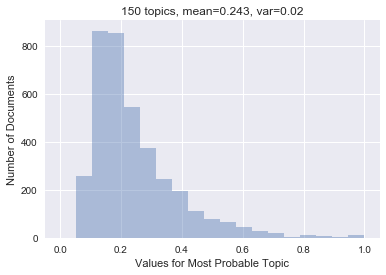
\includegraphics[width=6cm]{gfx/Hyperparams/150topics_English_nmf.png}
		\caption{Count of the value of the most probable topic, summed over all topics.}
		\label{fig:mean}%
	\end{minipage}%
	\begin{minipage}[b]{0.5\textwidth}
		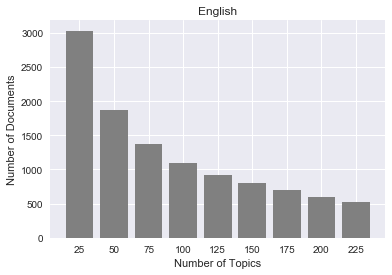
\includegraphics[width=6cm]{gfx/Hyperparams/English_nmf_Comments.png}
		\caption{Number of documents the topics are expressed above the threshold}
		\label{fig:topic number}
	\end{minipage}%
\end{figure}	

After finding the appropriate topic number, the Topic Models generated with \ac{NMF} and \ac{LDA} for the same dataset were inspected manually. The domain experts labeled the topics and the Topic Model with the higher number of labels was chosen. The final selection of the Topic Models is shown in Table \ref{tab:finaltopics_editorial_forums}. And the Topic Models for the summarized comments is shown in Table \ref{tab:editoria_comments}. \\


%Editorial and Forums
\begin{table}[h]
	\centering
	\makebox[0pt][c]{\parbox{1.0\textwidth}{%
		\begin{minipage}[b]{0.5\textwidth}
			\begin{tabular}[b]{lcc}
				\cmidrule{2-3}  & Editorial articles & Comments
				\\ \midrule
				German    & \textbf{190} &    \textit{125}       \\
				English    & \textbf{130}  &      \textbf{125}       \\ 
				\bottomrule
			\end{tabular}
		\end{minipage}
		\hfill
		%TODO welche Kommentare nmf oder lda wurden gewählt?
		\begin{minipage}[b]{0.5\textwidth}
			\begin{tabular}[b]{lccc}
				\cmidrule{2-4}  & \multicolumn{2}{c}{Editorials} & \multirow{2}{*}{Forums} \\
				\cmidrule(r){2-3}
				\cmidrule(r){2-3}
				& articles     &    comments       &                         
				\\ \midrule
				& \textbf{190} &  \textit{170}    &      \textit{170}       \\
				& \textbf{130} &  \textit{170}    &      \textbf{110}       \\ 
				\bottomrule
			\end{tabular}
		\end{minipage}
\vspace{1pt}
\caption[Final number of topics for Editorials and Forums]{The optimal number of topics for Editorials and Forums. \\
	\textit{Italic} denotes \ac{NMF} and \textbf{bold} numbers denote \ac{LDA}.}
\label{tab:finaltopics_editorial_forums}
}}
\end{table}

\chapter{Experiments and Evaluation}
\section{Topic ranking}


\subsection{Related work}

\subsection{Topic Coherence}

%document topic matrix theta
\subsection{Theta}

\subsection{Iterrater reliability}

%%rel work
% sumeed up theta
% vis doc topic visualization
%coherence



\section{Automatic Topic Labeling}
\label{kap:automaticTL}
%Topics are multinomial distributions a set of recurring themes that are discussed in the collection.

%Topics are a set of recurring themes that are discussed in the collection and represent as a multinomial distribution. Often the top words of the distribution is taken to represent

%of topic modeling can be used. Topic models refer to a set of algorithms that discoverthe topics or hidden thematic structure in a collection of documents. A topic modeltakes a set of documents as the input and outputs topics, a set of recurring themesthat are discussed in the collection, and the degree to which each document expressthese topics (Blei, 2012b). The results of the topic modeling algorithms can be usedto organize, visualize, summarize, and understand large collections of documents.

%A topic is commonly understood to be a a phrase or subject that best describesthe content of a text. In contrast, in topic modeling, every topic is a probabilitydistribution over all words in the collection of documents. In each topic a differentset of words has a high probability and we visualize the topic by listing the mostprobable terms.

Topic Models are used to discover latent topics in a corpus to help to understand large collections of documents. These topics are multinomial distributions over all words in a corpus. Normally the top terms of the distribution are taken to represent a topic but these words are often not helpful to interpret the coherent meaning of the topic. Especially, if the person is not familiar with the source collection.
With the help of Automatic Topic Labeling (\ac{ATL}) we want to reduce the cognitive overhead of interpreting these topics and therefore facilitate the interpretation of the topics.
Of course, the topics can be labeled manually by domain experts but this method is time consuming if there are hundreds of topics. Additionally, the topic labels can be biased towards the users opinion and the results are hard to replicate. \\
%%TODO human turks?
We are working with domain specific data dealing with organic food. To generate meaningful labels we can not make use of human turks but we need domain experts who are proficient in this area. Therefore we submitted the topics to our domain experts to label them. But only 50 of the generated topics for each dataset were handed in, in order to not burden them, since this process is very time-consuming. The datasets were labeled by three labelers who tried to find a suitable label, which captures the meaning of the topic and is easily understandable. After labeling every dataset the three labels were compared and a final label was set. If at least two labelers had the same label, this was taken as the final one. If the given labels were not comparable, no label was set at all. \\
To relieve our domain experts in the following chapter two approaches of \ac{ATL} are described. In Section \ref{sec:intrinsic} an intrinsic method was used, which is only working on texts and topics from our datasets to generate the labels according \cite{Mei2007}. Section \ref{sec:extrinsic} describes an extrinsic approach by using a lexical database for the English language called \textit{Wordnet} to label the topics.
 
%The domain experts labeled our topics. There were three labelers who tried to find a suitable label, which captures the meaning of the topic and is easily understandable. After labeling every dataset the three labels were compared and a final label was set. If at least two labelers had the same label, this was taken as the final one. If the given labels were not comparable, no label was set at all.\\


\subsection{Related work}                                                
\label{sec:relWorl: atl}
\textit{\cite{Lau2011}} generated a label set out of the article titles which were found in Wikipedia or Google by searching the top N words from the topics, called primary candidate labels. Afterwards, these were chunkized and n-grams were generated, which were searched in Wikipedia and Google. Theses secondary candidate labels were then filtered with the \textit{related article conceptual overlap} (RACO), that removed all outlier labels, like stop words. Then the primary and secondary candidate labels were ranked by features like \ac{PMI}, used for measuring association, and the student’s t test. The results were measured with the mean absolute error score for each label, which is an average of the absolute difference between an annotator’s rating and the average rating of a label, summed across all labels. The score lay between 0.5 and 0.56 on a scale from 0 to infinity.

On topics from Twitter \textit{\cite{Zhao2011}} used  a topic context sensitive Page Rank to find keywords by boosting the high relevant words to each topic. These keywords were taken to find keyword combinations (key phrases) that occur frequently in the text collection. The key phrases were ranked according to their relevance,i.e. whether they are related to the given topic and discriminative, and interestingness, the re-tweeting behavior in Twitter. To evaluate the key words Cohen’s Kappa was used to calculate the iterrater reliability between manually and automatically generated key phrases. The Cohen’s Kappa coefficient was in the range from 0.45 to 0.80, showing good agreement.

\textit{\cite{Allahyari2015}} created a topic model OntoLDA which incorporates an ontology into the topic model and provides \ac{ATL} too. In comparison with \ac{LDA}, OntoLDA has an additional latent variable, called concept, between topics and words. So each document is a multinational distribution over topics, each topic is a multinomial distribution over concepts and each concept is a multinomial distribution over words.  Based on the semantics of the concepts and the ontological relationships among them the labels for the topics are generated in followin steps:
\begin{description}
	\item (1) construction of the semantic graph from top concepts in the given topic
	\item (2) selection and analysis of the thematic graph (subgraph form the semantic graph)
	\item (3) topic graph extraction from the thematic graph concepts
	\item (4) computation of the semantic similarity between topic and the candidate labels of the topic label graph
\end{description}
The top N labels were compared with the labeling from \textit{\cite{Mei2007}} by calculating the precision after categorizing the labels into good and unrelated. The more labels were generated for a topic the more imprecise they got but the preciser \textit{\cite{Mei2007}} labels were.

\textit{\cite{Hulpus2013}} made use of the structured data from DBpedia, that contains structured information from Wikipedia. For each word of the topic the Word-sense disambiguation (WSD) chose the correct sense for the word from a set of different possible senses. Then a topic graph was obtained form DBpedia consisting of the closest neighbors and the links between the correct senses. Assuming the topic senses which are related, lie close to each other, different centrality measures were used and evaluated manually to identify the topic labels. The final labels then were compared to textual based approaches and the precision after categorizing the labels into good and unrelated was calculated.

\cite{Kou2015} captured the correlations between a topic and a label by calculating the cosine similarity between pairs of topic vectors and candidate label vectors. CBOW, Skip-gram and Letter Trigram Vectors were used. The candidate labels were extracted from Wikipedia articles that contained at least two of the top N topic words. The resulting labels for the different vector spaces were compared to automatically generated gold standard labels, representing the most frequent chunks of suitable document titles for a topic. The final labels were ranked by human annotators,too, and were considered as a better solution than the first word of the top N topic words. 

For topics and preprocessed Wikipedia titles \textit{\cite{Bhatia2016}} used word and title embeddings for both, generated by either doc2vec(for fine-grained labels) or word2vec (for generic labels), to generate topic labels. The relevance of each title embedding was measured with the pairwise cosine similarity of the word embeddings for the top N topic words. The sum of of the relevance of doc2vec and vec2doc served as ranking for the labels. The results were evaluated the same way like in \cite{Lau2011}.

\textit{\cite{Magatti2009}} used a given tree-structured hierarchy from the Google Directory to generate candidate labels for the topics. These were compared with the topic words applying different similarity measures showing a coherent behavior with respect to the semantics of the compared concepts. The most suitable label was then selected by exploiting a set of labeling
rules. This approach is applicable to any topic hierarchy summarized through a tree. The resuts were promising.

\textit{\cite{Mei2007}} generated labels based on the texts collection and their related topics by chunking and building n-grams. They approximated the distribution for the labels and compared these to the distribution of the topic by calculating the \ac{KL} divergence. To maximize the mutual information between the label and the topic distributions the calculated divergence has to be minimized. Three human assessors measured the results and found out that the final labels are effective and robust although applied on different genres of text collections. 


\subsection{Intrinsic Topic Labeling}
\label{sec:intrinsic}
The intrinsic topic labeling is only based on the text collection and the extracted topics and does not use any external ontologies or embeddings. Because \textit{\cite{Mei2007}} were the only ones who generated topic labels by using an intrinsic approach, we decided to apply their \ac{ATL} on our data, using the implementation from Github\footnote{https://github.com/xiaohan2012/chowmein}. 

In their paper \textit{\cite{Mei2007}} consider noun phrases and n-grams as candidate labels and use \ac{POS}-tags to extract the label according to some grammar from the text collection. We apply the n-grams approach to select (NN - NN) or (JJ - NN) English and (NN -NN) or (ADJD - NN) German bi-grams as suitable labels for the topics.

The candidate labels were ranked by their semantical similarity to the topic model $\theta$. To measure the semantic relevance between the topic and the label \textit{l} a distribution of words \textit{w} for the label $p(w|l)$ was approximated by including a text collection \textit{C} and a distribution $p(w|l,C)$ was estimated, to substitute $p(w|l)$. Then the \ac{KL} divergence $D(\theta||l)$ was applied to calculate the closeness between the label and the topic distribution $p(w|\theta)$. So the \ac{KL} divergence served to capture how well the label fits to our topic. If the two distributions perfectly match each other and the divergence is zero we have found the best label. 
The relevance scoring function of \textit{l}  to $\theta$ is defined as the negative \ac{KL} divergence $-D(\theta||l)$ of $p(w|\theta)$ and $p(w|l)$ and can be rewritten as follows by including \textit{C}:
\begin{align}
\begin{split}
	Score(l,\theta) = &-D(\theta||l) =
	-\sum_{w} p(w|\theta)log\frac{p(w|\theta)}{p(w|l)}\\ =
	&-\sum_{w} p(w|\theta)log\frac{p(w|C)}{p(w|l,C)} -\sum_{w} p(w|\theta)log\frac{p(w|\theta)}{p(w|l)}\\ &-\sum_{w} p(w|\theta)log\frac{p(w|l,C)}{p(w|l)} \\ =
	&-\sum_{w} p(w|\theta)log\frac{p(w,l|C)}{p(w|C) p(l|C)} -D(\theta||C)\\ &-\sum_{w} p(w|\theta)log\frac{p(w|l,C)}{p(w|l)}\\  =
	&-\sum_{w} p(w|\theta) PMI(w,l|C)-D(\theta||C) + Bias(l|C) 
\end{split}
\end{align}
We can see that the relevance scoring function consists of three parts. The first part represents the expectation of \ac{PMI} $E_{\theta}(PMI(w,l|C))$ between \textit{l} and the words in the topic model given the context \textit{C}, the second part by the \ac{KL} divergence between $\theta$ and \textit{C} and the third part can be viewed as a bias using context
\textit{C} to infer the semantic relevance \textit{l} and $\theta$. This bias can be neglected for our data because we have used the same text collection for  producing the topics and the labels. The same applies to the second part, because the \ac{KL} divergence has the same value for all candidate labels. Therefore, we rank the topic labels with 
\begin{equation}
Score(l,\theta) = E_{\theta}(PMI(w,l|C))
\label{Mei:Scoring}
\end{equation}

\begin{figure}[t]
	\begin{minipage}[t]{0.5\textwidth}
		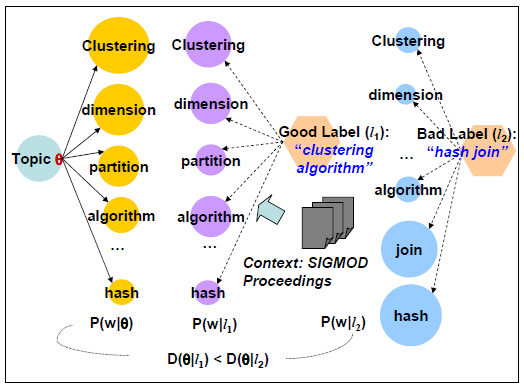
\includegraphics[width=\textwidth]{gfx/Mei/MeiGoodLabel.png}
	\end{minipage}
	\begin{minipage}[t]{0.512\textwidth}
		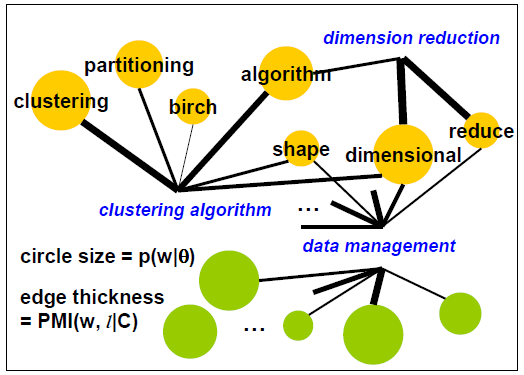
\includegraphics[width=\textwidth]{gfx/Mei/MeiScoring.png}
	\end{minipage}
	\caption[Relevance scoring function for \ac{ATL}]{Relevance scoring function for \ac{ATL}. Adapted from \cite{Mei2007}}
	\label{pic:ScoringFunction}
\end{figure}

The relevance scoring function is also described visually in Figure \ref{pic:ScoringFunction}. The circles represent the probability of terms. The larger the circle the higher is the probability. On the left one can see that the label with lower \ac{KL} divergence is the best one. To approximate $p(w|l)$ the \textit{SIGMOD Proceedings} were used as the text collection \textit{C}. Analogously, we used our datasets. On the right one can a weighted graph, where each node is a term in the topic model $\theta$ and the edges between terms and the label are weighted by their \ac{PMI}. The weight of the node indicates the importance of a term to the topic, while the weight of each edge indicates the semantical strength between label and term. The relevance scoring function ranks a node higher if the label has a strong semantic relation to the important topical words. Visually, this can be understood that the label is ranked higher if it connects to large circle by a thick edge.

So far only the labeling of a topic was considered, but a characteristic of a good label is the discrimination towards other topics in the topic model,too. It is not useful if many topics have the same labels, although it may be a good label for the topic individually, because we can not make differentiations between the topics. The label should have a high semantic relevance to a topic and low relevance to other topics. In order to take this property into account the $Score(l,\theta)$ in \ref{Mei:Scoring} was adjusted to: 
\begin{equation}
Score'(l,\theta_{i}) = Score(l,\\theta_{i}) - \mu Score(l,\theta_{1,...,i-1,i+1,...})
%Score(l,\theta) = (1+\dfrac{\mu}{k-1}) E_{\theta_{i}}(PMI(w,l|C)) - \dfrac{\mu}{k-1} \sum_{j=1...k} %E_{\theta_{j}}(PMI(w,l|C))
\end{equation}
$\theta_{1,...,i-1,i+1,...}$ describes all topics except the $\theta_{i}$ and $\mu$ controls the discriminative power.

%The semantic relevance function already guarantees that the label covers the maximal semantic information of $\theta$. Even though one label covers only a topic partially. So a selection of multiple labels for a topic shall cover different aspects of the topic. This is called the intra-topic coverage. For the selection of labels the Maximal Marginal Relevance (MMR) (\cite{Carbonell1998}) was used to get high relevant and low redundant labels.
\subsubsection{Evaluation}
We applied the \ac{ATL} according \cite{Mei2007} on the Dataset \ref{chris:daten}. 


 



%changed the implementation, used our preprocessing(stop words)
%made postagging on our data 
%without bigramms
%with bigrams
%with postags
%candidate label generation:

%	Code: Candidate phrase detection using pointwise mutual information: POS tag constraint can be applied. For now, only bigrams are considered.

%	Changes: 
%		-our vectorizer, 
%		nope-throw out words which are smaller then 3 characters
%		-used our preprocessing
%		- generated our own postags on the data
	
	
\subsection{Extrinsic Labeling}
\label{sec:extrinsic}

\footnote{http://www.nltk.org/howto/wordnet.html}
%

\textbf{Chapter \ref{sec:related}} \\[0.2em]
\blindtext

\section{Intern Consistency}

\chapter{Future Work and Conclusion}

\section{Future work}

\section{Conclusion}

 % Weitere Kapitel hier einfügen 

% --------------------------
% Back matter
% --------------------------
\appendix\cleardoublepage
% !TEX root = ../my-thesis.tex
%
\chapter{Descriptive Statistics of the Dataset}
\label{app:descriptiv_stats}
\begin{figure}[h]
	\begin{center}
		%
		\subfloat[Number of Articles per Type]{%
			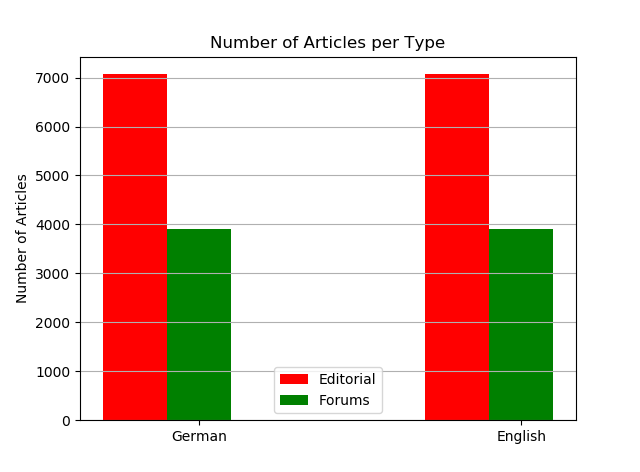
\includegraphics[width=0.5\textwidth]{gfx/descriptive_statistics/Number_of_articles_per_type.png}
		}%
		\subfloat[Number of Comments per Type]{%
			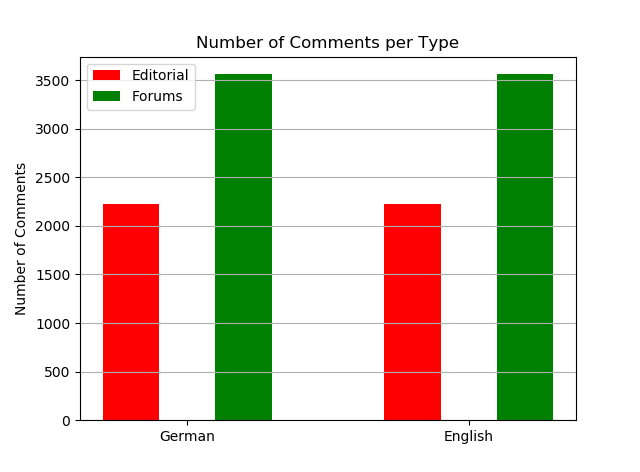
\includegraphics[width=0.5\textwidth]{gfx/descriptive_statistics/Number_of_comments_per_type.png}
		}\\ %  ------- End of the first row ----------------------%
		\subfloat[Distribution of English articles per year]{%
			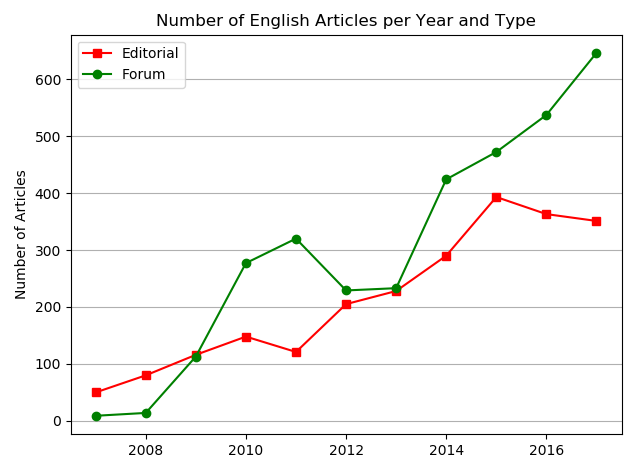
\includegraphics[width=0.5\textwidth]{gfx/descriptive_statistics/Number_of_english_articles_per_year_and_type.png}
		}%
		\subfloat[Distribution of German articles per year]{%
			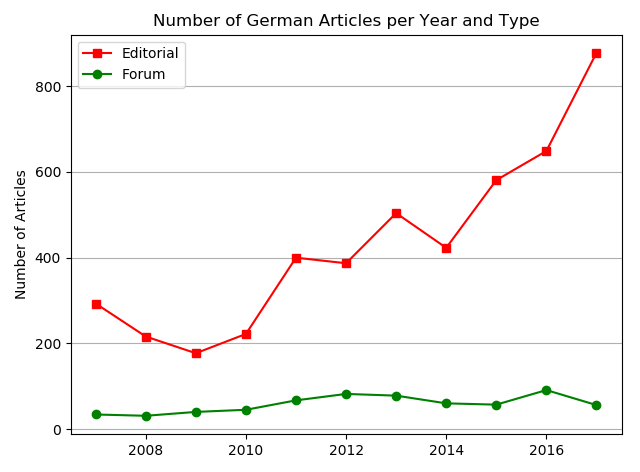
\includegraphics[width=0.5\textwidth]{gfx/descriptive_statistics/Number_of_Germna_articles_per_year_and_type.png}
		}%
		%
	\end{center}
	\caption{Descriptive Statistics for all datasets}
	\label{fig:descriptive_stats}
\end{figure}

\section{Detailed Statistics of all Sources}
% English Editorial
\begin{sidewaystable}
	\begin{tabular}{lrrrrrr}
		\toprule
		Source           & Total articles & Relevant articles & \% rel. articles & Avg. article length\footnotemark[1] & Rel. art. w/ cmnt. & \% rel. art. w/ cmnt. \\ \midrule
		usatoday         &             95 &                61 &            64.21 &                 303 &                 15 &                 24.59 \\
		nytimes          &            438 &               327 &            74.66 &                 528 &                 99 &                 30.28 \\
		nypost           &            106 &                33 &            31.13 &                 377 &                  0 &                  0.00 \\
		washingtonpost   &           1563 &               489 &            31.29 &                 480 &                285 &                 58.28 \\
		latimes          &           1522 &               270 &            17.74 &                 419 &                  8 &                  2.96 \\
		chicagotribune   &           2283 &               572 &            25.05 &                 420 &                 39 &                  6.82 \\
		huffingtonpost   &            880 &               668 &            75.91 &                 479 &                  0 &                  0.00 \\
		organicauthority &             66 &                43 &            65.15 &                 626 &                  0 &                  0.00 \\ \bottomrule
	\end{tabular}
	\caption{Article statistics for English editorial data} 
	\begin{tabular}{lrrrrrrr}
		\toprule
		Source           & Total comments & Relevant comments & \% rel. cmnt. & Root cmnt. & \% root cmnt. & Avg. \# cmnt. & Avg. cmnt. length\footnotemark[1] \\ \midrule
		usatoday         &            259 &               195 &         75.29 &        103 &         52.82 &             3 &                17 \\
		nytimes          &          16128 &             11576 &         71.78 &       7353 &         63.52 &            35 &                40 \\
		nypost           &              0 &                 0 &          0.00 &          0 &          0.00 &             0 &                 0 \\
		washingtonpost   &          84669 &             14875 &         17.57 &       6667 &         44.82 &            30 &                24 \\
		latimes          &            374 &                14 &          3.74 &         12 &         85.71 &             0 &                34 \\
		chicagotribune   &            281 &               154 &         54.80 &        131 &         85.06 &             0 &                19 \\
		huffingtonpost   &              0 &                 0 &          0.00 &          0 &          0.00 &             0 &                 0 \\
		organicauthority &              0 &                 0 &          0.00 &          0 &          0.00 &             0 &                 0 \\ \bottomrule
	\end{tabular}
	
	\caption{Comment statistics for English editorial data} 
\end{sidewaystable}

% English forums
\begin{sidewaystable}
	\begin{tabular}{lrrrrrr}
		\toprule
		Source         & Total articles & Relevant articles & \% rel. articles & Avg. article length\footnotemark[1] & Rel. art. w/ cmnt. & \% rel. art. w/ cmnt. \\ \midrule
		reddit         &            256 &               225 &            87.89 &                  49 &                190 &                 84.44 \\
		usmessageboard &            382 &                61 &            15.97 &                   0 &                 61 &                100.00 \\
		cafemom        &             88 &                26 &            29.55 &                 251 &                 26 &                100.00 \\
		quora          &           1703 &              1497 &            87.90 &                   5 &               1304 &                 87.11 \\
		fb             &           5035 &              1467 &            29.14 &                  23 &               1355 &                 92.37 \\ \bottomrule
	\end{tabular}
	
	\caption{Article statistics for English forum data} 
	\begin{tabular}{lrrrrrrr}
		\toprule
		Source         & Total comments & Relevant comments & \% rel. cmnt. & Root cmnt. & \% root cmnt. & Avg. \# cmnt. & Avg. cmnt. length\footnotemark[1] \\ \midrule
		reddit         &           9291 &              8392 &         90.32 &       1574 &         18.76 &            37 &                25 \\
		usmessageboard &          78303 &              1982 &          2.53 &       1254 &         63.27 &            32 &                43 \\
		cafemom        &           2206 &               352 &         15.96 &        280 &         79.55 &            13 &                30 \\
		quora          &           9606 &              8699 &         90.56 &       5229 &         60.11 &             5 &                46 \\
		fb             &         299126 &             81660 &         27.30 &      64183 &         78.60 &            55 &                11 \\ \bottomrule
	\end{tabular}
	\caption{Comment statistics for English forum data} 
\end{sidewaystable}

\begin{sidewaystable}
	\begin{tabular}{lrrrrrr}
		\toprule
		Source             & Total articles & Relevant articles & \% rel. articles & Avg. article length\footnotemark[1] & Rel. art. w/ cmnt. & \% rel. art. w/ cmnt. \\ \midrule
		spiegel            &            468 &               152 &            32.48 &                 376 &                 61 &                 40.13 \\
		zeit               &            154 &                62 &            40.26 &                 461 &                 35 &                 56.45 \\
		welt               &            729 &               392 &            53.77 &                 323 &                 35 &                  8.93 \\
		taz                &           2458 &              1406 &            57.20 &                 255 &                249 &                 17.71 \\
		tagesspiegel       &            625 &               278 &            44.48 &                 279 &                 41 &                 14.75 \\
		handelsblatt       &            567 &               286 &            50.44 &                 302 &                 65 &                 22.73 \\
		freitag            &             16 &                 7 &            43.75 &                 678 &                  5 &                 71.43 \\
		tagesschau         &             61 &                17 &            27.87 &                 202 &                 17 &                100.00 \\
		br                 &            191 &                93 &            48.69 &                 297 &                 26 &                 27.96 \\
		wdr                &             68 &                37 &            54.41 &                 241 &                  0 &                  0.00 \\
		swr                &            164 &                82 &            50.00 &                 207 &                  0 &                  0.00 \\
		ndr                &             18 &                 5 &            27.78 &                 209 &                  0 &                  0.00 \\
		derstandard        &           1092 &               646 &            59.16 &                 231 &                529 &                 81.89 \\
		diepresse          &            304 &               152 &            50.00 &                 230 &                100 &                 65.79 \\
		kurier             &            287 &               165 &            57.49 &                 199 &                 88 &                 53.33 \\
		nachrichtenat      &            254 &               134 &            52.76 &                 198 &                 75 &                 55.97 \\
		salzburgcom        &            154 &                93 &            60.39 &                 177 &                  0 &                  0.00 \\
		krone              &             97 &                31 &            31.96 &                 143 &                  0 &                  0.00 \\
		tagesanzeiger      &            187 &                32 &            17.11 &                 171 &                 17 &                 53.12 \\
		nzz                &            316 &               108 &            34.18 &                 338 &                 17 &                 15.74 \\
		aargauer           &            110 &                46 &            41.82 &                 221 &                 17 &                 36.96 \\
		luzernzeitung      &            105 &                55 &            52.38 &                 217 &                  0 &                  0.00 \\
		srf                &            147 &                85 &            57.82 &                 194 &                 56 &                 65.88 \\
		forum\_ernaehrung  &             18 &                 3 &            16.67 &                 339 &                  0 &                  0.00 \\
		heise              &             33 &                17 &            51.52 &                 479 &                 17 &                100.00 \\
		eatsmarter         &            300 &               100 &            33.33 &                 176 &                 35 &                 35.00 \\
		huffingtonpost\_de &            293 &                94 &            32.08 &                 248 &                  0 &                  0.00 \\
		waz                &            744 &               207 &            27.82 &                 193 &                 68 &                 32.85 \\
		merkur             &            393 &               243 &            61.83 &                 209 &                 69 &                 28.40 \\
		rp                 &            604 &               267 &            44.21 &                 204 &                103 &                 38.58 \\
		focus              &            777 &               397 &            51.09 &                 176 &                154 &                 38.79 \\
		campact            &             61 &                23 &            37.70 &                 224 &                 23 &                100.00 \\ \bottomrule
	\end{tabular}
	\caption{Article statistics for German editorial data} 
\end{sidewaystable}

\begin{sidewaystable}	
	\begin{tabular}{lrrrrrrr}
		\toprule
		Source             & Total comments & Relevant comments & \% rel. cmnt. & Root cmnt. & \% root cmnt. & Avg. \# cmnt. & Avg. cmnt. length\footnotemark[1] \\ \midrule
		spiegel            &          62860 &             21551 &         34.28 &       5863 &         27.21 &           141 &                48 \\
		zeit               &           8496 &              2977 &         35.04 &       1279 &         42.96 &            48 &                32 \\
		welt               &           1448 &               528 &         36.46 &        316 &         59.85 &             1 &                21 \\
		taz                &           5537 &              2608 &         47.10 &       1310 &         50.23 &             1 &                28 \\
		tagesspiegel       &           3535 &              1279 &         36.18 &       1279 &        100.00 &             4 &                36 \\
		handelsblatt       &            923 &               295 &         31.96 &        222 &         75.25 &             1 &                28 \\
		freitag            &            129 &                65 &         50.39 &         33 &         50.77 &             9 &                34 \\
		tagesschau         &           4377 &               841 &         19.21 &        841 &        100.00 &            49 &                32 \\
		br                 &            386 &               343 &         88.86 &        220 &         64.14 &             3 &                26 \\
		wdr                &              0 &                 0 &          0.00 &          0 &          0.00 &             0 &                 0 \\
		swr                &              0 &                 0 &          0.00 &          0 &          0.00 &             0 &                 0 \\
		ndr                &              0 &                 0 &          0.00 &          0 &          0.00 &             0 &                 0 \\
		derstandard        &          80715 &             50790 &         62.93 &      12152 &         23.93 &            78 &                15 \\
		diepresse          &           3015 &              1796 &         59.57 &        891 &         49.61 &            11 &                22 \\
		kurier             &            870 &               471 &         54.14 &        308 &         65.39 &             2 &                17 \\
		nachrichtenat      &           1992 &               678 &         34.04 &        310 &         45.72 &             5 &                14 \\
		salzburgcom        &              0 &                 0 &          0.00 &          0 &          0.00 &             0 &                 0 \\
		krone              &              0 &                 0 &          0.00 &          0 &          0.00 &             0 &                 0 \\
		tagesanzeiger      &           4872 &              1139 &         23.38 &        664 &         58.30 &            35 &                18 \\
		nzz                &            622 &               162 &         26.05 &        101 &         62.35 &             1 &                32 \\
		aargauer           &            397 &               262 &         65.99 &        122 &         46.56 &             5 &                18 \\
		luzernzeitung      &              0 &                 0 &          0.00 &          0 &          0.00 &             0 &                 0 \\
		srf                &           1477 &               941 &         63.71 &        652 &         69.29 &            11 &                20 \\
		forum\_ernaehrung  &              0 &                 0 &          0.00 &          0 &          0.00 &             0 &                 0 \\
		heise              &           3636 &              1835 &         50.47 &        335 &         18.26 &           107 &                53 \\
		eatsmarter         &           1179 &               162 &         13.74 &        146 &         90.12 &             1 &                30 \\
		huffingtonpost\_de &              0 &                 0 &          0.00 &          0 &          0.00 &             0 &                 0 \\
		waz                &           1827 &               459 &         25.12 &        327 &         71.24 &             2 &                25 \\
		merkur             &            699 &               347 &         49.64 &        194 &         55.91 &             1 &                15 \\
		rp                 &           1808 &               822 &         45.46 &        822 &        100.00 &             3 &                35 \\
		focus              &           5806 &              2477 &         42.66 &       2123 &         85.71 &             6 &                24 \\
		campact            &           2577 &               687 &         26.66 &        518 &         75.40 &            29 &                30 \\ \bottomrule
	\end{tabular}
	\caption{Comment statistics for German editorial data} 
\end{sidewaystable}

\begin{sidewaystable}
	\begin{tabular}{lrrrrrr}
		\toprule
		Source             & Total articles & Relevant articles & \% rel. articles & Avg. article length\footnotemark[1] & Rel. art. w/ cmnt. & \% rel. art. w/ cmnt. \\ \midrule
		reddit\_de         &             83 &                44 &            53.01 &                   3 &                 33 &                 75.00 \\
		gutefrage          &            547 &               396 &            72.39 &                  17 &                396 &                100.00 \\
		werweisswas        &             33 &                27 &            81.82 &                  30 &                 26 &                 96.30 \\
		glamour            &              3 &                 2 &            66.67 &                  58 &                  2 &                100.00 \\
		webkoch            &              4 &                 3 &            75.00 &                 221 &                  2 &                 66.67 \\
		chefkoch           &            248 &               150 &            60.48 &                  54 &                150 &                100.00 \\
		paradisi           &             18 &                18 &           100.00 &                  19 &                 18 &                100.00 \\
		kleiderkreisel     &             69 &                24 &            34.78 &                  50 &                 24 &                100.00 \\
		biooekoforum       &              1 &                 1 &           100.00 &                  19 &                  1 &                100.00 \\
		bfriendsBrigitte   &             20 &                11 &            55.00 &                  56 &                 11 &                100.00 \\
		schule-und-familie &              2 &                 2 &           100.00 &                  32 &                  1 &                 50.00 \\ \bottomrule
	\end{tabular}
	
	\caption{Article statistics for German forum data} 
	\begin{tabular}{lrrrrrrr}
		\toprule
		Source             & Total comments & Relevant comments & \% rel. cmnt. & Root cmnt. & \% root cmnt. & Avg. \# cmnt. & Avg. cmnt. length\footnotemark[1] \\ \midrule
		reddit\_de         &           1665 &               488 &         29.31 &        138 &         28.28 &            11 &                16 \\
		gutefrage          &           6005 &              4100 &         68.28 &       1898 &         46.29 &            10 &                19 \\
		werweisswas        &            241 &               195 &         80.91 &        195 &        100.00 &             7 &                39 \\
		glamour            &            287 &               188 &         65.51 &        188 &        100.00 &            94 &                29 \\
		webkoch            &             34 &                34 &        100.00 &         34 &        100.00 &            11 &                22 \\
		chefkoch           &           9804 &              5750 &         58.65 &       5750 &        100.00 &            38 &                36 \\
		paradisi           &             63 &                63 &        100.00 &         63 &        100.00 &             3 &                17 \\
		kleiderkreisel     &           4831 &              1255 &         25.98 &        854 &         68.05 &            52 &                18 \\
		biooekoforum       &             15 &                15 &        100.00 &         15 &        100.00 &            15 &                23 \\
		bfriendsBrigitte   &           2898 &               740 &         25.53 &        740 &        100.00 &            67 &                37 \\
		schule-und-familie &             28 &                28 &        100.00 &         28 &        100.00 &            14 &                31 \\ \bottomrule
	\end{tabular}	
	\caption{Comment statistics for German forum data} 
\end{sidewaystable}
\footnotetext[1]{The average number of tokens after lemmatizing and stop word removal.}
\section{JSON Storage Schema}
\label{sec:appendix:json}
\begin{center}
	\begin{listing}
		\begin{minted}[linenos,tabsize=3,breaklines]{json}
			{
				"article_title":"article title",
				"article_author":[
				{
					"article_author_id":"123456789",
					"article_author_name":"author name"
				}
				],
				"article_time":"2015-10-17 20:02:54",
				"article_text":"article text",
				"article_source":"news source",
				"comments":[
				{
					"comment_id":"123456789",
					"comment_author": {
						"comment_author_id":"45678",
						"comment_author_name":"author name",
					},
					"comment_time":"2015-10-20 04:17:17",
					"comment_text":"comment text",
					"comment_rating":-15.0,
					"comment_title":"example title"
				},
				{
					"comment_id":"987654321",
					"comment_author":{
						"comment_author_id":"12345",
						"comment_author_name":"author name"
					},
					"comment_time":"2015-10-19 19:16:33",
					"comment_text":"comment text",
					"comment_replyTo":"123456789",
					"comment_rating":6.0
				}
				],
				"search_query":"organic farming",
				"article_url":"https://example.url",
				"resource_type":"editorial | blog | forum",
				"article_rating":5.0
			}
		\end{minted}
		\caption{JSON Storage Schema}
		\label{jsonschema}
	\end{listing}
\end{center}
       % INCLUDE: appendix
%
{%
\setstretch{1.1}
\renewcommand{\bibfont}{\normalfont\small}
\setlength{\biblabelsep}{0pt}
\setlength{\bibitemsep}{0.5\baselineskip plus 0.5\baselineskip}

\printbibliography[nottype=online]
\printbibliography[heading=subbibliography,title={Webpages},type=online,prefixnumbers={@}]
}
\cleardoublepage

\listoffigures
\cleardoublepage

\listoftables
\cleardoublepage
% **************************************************
% End of Document CONTENT
% **************************************************
\end{document}
